\documentclass[12pt,twosize,openany]{book}
\usepackage[cp866]{inputenc}           % Перешли на кодировку Windows!!!
\usepackage[english, russian]{babel}    % Переносы через Babel (обязательно!)
\usepackage[dvips]{graphicx}
\usepackage{amsmath}
\usepackage{amssymb}
\usepackage{amsthm}
\usepackage[dvips]{color}
\usepackage{colordvi}
\usepackage{graphicx}
\usepackage{ifpdf}
\ifpdf \DeclareGraphicsRule{*}{mps}{*}{} \fi
\usepackage{srcltx}

\begin{document}
\vspace{5cm}

\thispagestyle{empty}
\begin{center}
{\Huge{\textbf{ИЗЛОЖЕНИЕ ЛЕКЦИЙ }}}\\[10pt]

{\Huge{\textbf{С.\,Б.\,СТЕЧКИНА}}}\\[10pt]
\end{center}

{\Huge{\textbf{\hspace{-0.5cm}ПО ТЕОРИИ ПРИБЛИЖЕНИЙ}}}\\[10pt]

%{\Huge{\textbf{ПРИБЛИЖЕНИЙ}}}\\


\vspace{2cm}

\begin{figure}[ht]
\begin{center}
\includegraphics[width=0.8\textwidth]{pict/moln-2.5.eps}
\end{center}
 \bigskip
 \end{figure}

\end{document}
